\documentclass[tikz]{standalone}
\usetikzlibrary{intersections}
\begin{document}
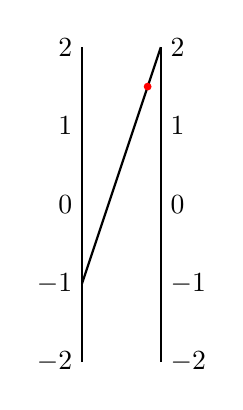
\begin{tikzpicture}
  \draw[thick] (0, -2) -- (0, 2) node[above] {};
  \draw[thick] (1, -2) -- (1, 2) node[above] {};

  \foreach \y in {-2, -1, 0, 1, 2} {
      \node[left] at (0, \y) {$\y$};
      \node[right] at (1, \y) {$\y$};
  }

  \draw[thick] (0,-1) -- (1,2) node {};
  \node[circle,fill,color=red,inner sep=1pt] at (0.833, 1.5) {};
\end{tikzpicture}
\end{document}
